
\chapter{Results} \label{chap:result}

\section{Method}

For benchmarking two metrics were measured:

\begin{itemize}
	\item \textbf{Time} \\
	      Seconds until a solution is found.
	\item \textbf{Iterations} \\
	      How many times the recursive algorithm was called.
\end{itemize}

For Time measurements hyperfine~\cite{hyperfine:2023} is used. Each Time Benchmark includes 3 warm up runs and is averaged. The longer the solver takes, the fewer runs are done. This is default behavior of hyperfine. However, at least 10 runs made were made for each benchmark. Time is given in seconds. Iterations were measured by doing 5 runs and averaging them.

A benchmark is a pair of problem size with a combination of algorithmic modifications to the solver. As Oxiflex allows us to enable each optimization individually, we can create 8 optimization combinations.

\begin{itemize}
	\item \verb|-n -r| \\
	      NaiveBacktracking
	\item \verb|-n| \\
	      NaiveBacktracking with variable ordering
	\item \verb|-f -r| \\
	      Inference with forward checking
	\item \verb|-f| \\
	      Inference with forward checking and variable ordering
	\item \verb|-a 1 -r| \\
	      Inference with AC-1
	\item \verb|-a 1| \\
	      Inference with AC-1 and variable ordering
	\item \verb|-r| \\
	      Inference with AC-3
	\item \verb|no flags| \\
	      Inference with AC-3 and variable ordering
\end{itemize}

The following Problem Domains where measured:

\begin{itemize}
	\item N-Queens
	\item Slow Convergence
\end{itemize}

All benchmarks were performed on the same machine. \\

\begin{tabular}{>{\hspace{1em}}l l}
	CPU:               & Intel i7-6700K (8) @ 4.200GHz \\
	Memory:            & 6051MiB / 32021MiB            \\
	hyperfine version: & 1.16.1                        \\
	Rust version:      & 1.76.0                        \\
	Operating System:  & Pop!\_OS 22.04 LTS
\end{tabular}

\section{N-Queens}

\cref{fig:queens:time}\footnote{ChatGPT 4 was used to help write scripts that create the plots. \url{https://chatgpt.com}} shows the runtime comparison for the N-Queens Problem (See~\cref{sec:queens}:~\nameref{sec:queens}) with $n = 8..20$ for all combinations. It shows that arc consistency enforcing methods AC-1 and AC-3 in Oxiflex take much more Time then the naive and forward checking approach. We can also see that variable ordering seems to improve all approaches significantly.

\begin{figure}[ht]
	\centering
	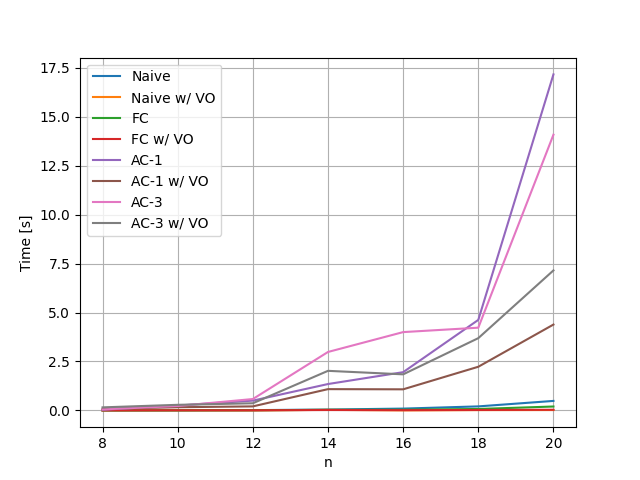
\includegraphics[width=0.8\textwidth]{./Problems/queens/plots/time.png}
	\caption{N-Queen Time measurements averaged over multiple runs (at least 10).}
	\label{fig:queens:time}
\end{figure}

\cref{fig:queens:time-no-arc} does not include arc consistency enforcing methods making it clear to see the impact of forward checking on Time measurements for the N-Queens Problem. This shows that although the naive approach without variable ordering performs much worse then forward checking without variable ordering, it outperforms forward checking with variable ordering.

\begin{figure}[ht]
	\centering
	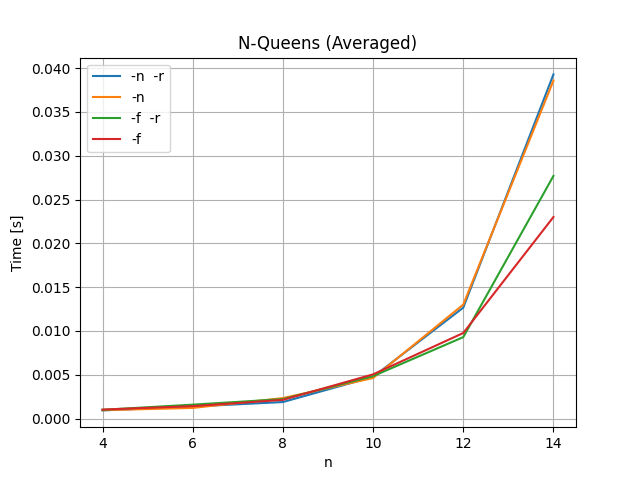
\includegraphics[width=0.8\textwidth]{./Problems/queens/plots/time_no_arc.png}
	\caption{N-Queens Time measurements without arc consistency averaged over multiple runs (at least 10).}
	\label{fig:queens:time-no-arc}
\end{figure}

\cref{fig:queens:iterations} shows benchmarks with the same parameters for measurements of Iterations. It shows that the number of Iterations grows significantly up from $n = 20$. And although we could see that arc consistency enforcing methods worsen the performance Time wise, they provide huge improvements for number of Iterations.

\begin{figure}[ht]
	\centering
	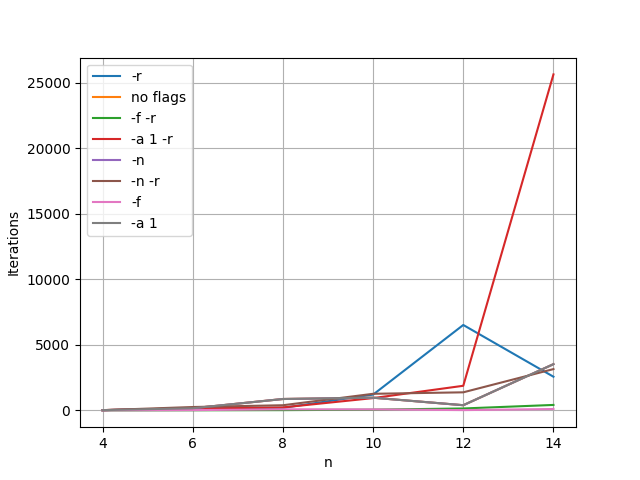
\includegraphics[width=0.8\textwidth]{./Problems/queens/plots/iterations.png}
	\caption{N-Queens iteration measurements averaged over 5 runs.}
	\label{fig:queens:iterations}
\end{figure}

In \cref{fig:queens:iterations-inference} we provide benchmarks for Iterations without the naive approach with $n = 14$ up to $n = 24$. As expected forward checking performed the worst out of the three.

\begin{figure}[ht]
	\centering
	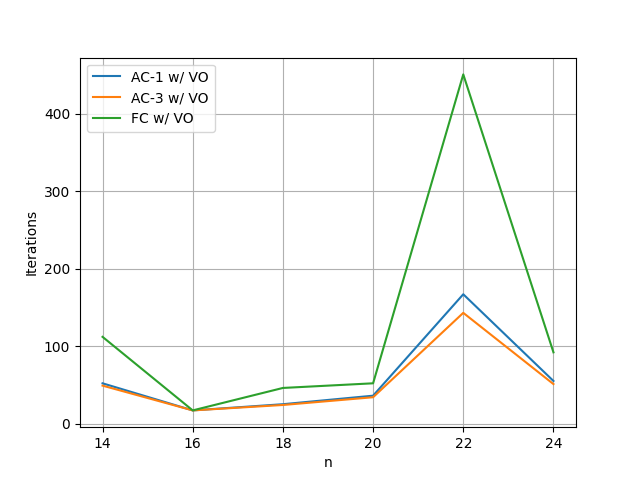
\includegraphics[width=0.8\textwidth]{./Problems/queens/plots/iterations_inference.png}
	\caption{N-Queens Iterations only inference averaged over 5 runs.}
	\label{fig:queens:iterations-inference}
\end{figure}

Table~\ref{tab:queens:time} and Table~\ref{tab:queens:iterations} contain results for Time and Iterations including standard deviation. Time values are rounded to 2 decimal places. If there is a standard deviation for the measurements it is given after the $\pm$ symbol. If there is no variable ordering the measurements can vary greatly because variables are chosen randomly to be assigned a value.

\begin{table}[h!]
	\centering
	\begin{tabular}{|c|c|c|c|c|c|c|}
		\hline
		$n$         & 14              & 16              & 18              & 20                \\ \hline
		Naive       & 0.05 $\pm$ 0.08 & 0.09 $\pm$ 0.12 & 0.21 $\pm$ 0.45 & 0.49 $\pm$ 1.29   \\ \hline
		FC          & 0.03 $\pm$ 0.03 & 0.04 $\pm$ 0.04 & 0.07 $\pm$ 0.10 & 0.20 $\pm$ 0.66   \\ \hline
		AC-1        & 1.35 $\pm$ 0.73 & 1.95 $\pm$ 1.06 & 4.62 $\pm$ 3.25 & 17.17 $\pm$ 31.87 \\ \hline
		AC-3        & 2.99 $\pm$ 1.92 & 4.00 $\pm$ 2.67 & 4.23 $\pm$ 0.97 & 14.09 $\pm$ 9.93  \\ \hline
		Naive w/ VO & 0.03            & 0.00            & 0.02            & 0.02              \\ \hline
		FC w/ VO    & 0.02            & 0.01            & 0.02            & 0.03              \\ \hline
		AC1 w/ VO   & 1.09 $\pm$ 0.02 & 1.08 $\pm$ 0.03 & 2.23 $\pm$ 0.04 & 4.39 $\pm$ 0.06   \\ \hline
		AC3 w/ VO   & 2.02 $\pm$ 0.04 & 1.84 $\pm$ 0.05 & 3.69 $\pm$ 0.06 & 7.15 $\pm$ 0.05   \\ \hline
	\end{tabular}
	\caption{N-Queens Time in seconds averaged over multiple runs (at least 10), Mean$\pm$SD, w/ VO: with variable ordering.}
	\label{tab:queens:time}
\end{table}

\begin{table}[h!]
	\centering
	\begin{tabular}{|c|c|c|c|c|c|c|}
		\hline
		$n$         & 14              & 16             & 18              & 20                \\ \hline
		Naive       & 3538 $\pm$ 1148 & 1749 $\pm$ 907 & 2760 $\pm$ 1145 & 21479 $\pm$ 11183 \\ \hline
		FC          & 110 $\pm$ 51    & 415 $\pm$ 76   & 79 $\pm$ 16     & 270 $\pm$ 63      \\ \hline
		AC-1        & 51 $\pm$ 9      & 396 $\pm$ 343  & 195 $\pm$ 67    & 104 $\pm$ 19      \\ \hline
		AC-3        & 103 $\pm$ 41    & 34 $\pm$ 6     & 91 $\pm$ 68     & 86 $\pm$ 30       \\ \hline
		Naive w/ VO & 3536            & 137            & 1018            & 1011              \\ \hline
		FC w/ VO    & 112             & 17             & 46              & 52                \\ \hline
		AC1 w/ VO   & 52              & 17             & 25              & 36                \\ \hline
		AC3 w/ VO   & 49              & 17             & 24              & 34                \\ \hline
	\end{tabular}
	\caption{N-Queens Iterations averaged over 5 runs, Mean$\pm$SD, w/ VO: with variable ordering.}
	\label{tab:queens:iterations}
\end{table}

\section{Slow Convergence}

The Slow Convergence Problem is from the MiniZinc benchmarks repository~\cite{minizinc_slow:2018}. Benchmarks for this problem without variable ordering took over 300 seconds and are therefore omitted. \cref{fig:slow:time-small} shows benchmarks for $n=2..10$ with combinations using variable ordering. We can see that Time measurements for AC-1 and AC-3 grow exponentially and it seems that the naive and forward checking approach grow linearly.

\cref{fig:slow:iterations-small} shows benchmarks with the same parameters for measurements of Iterations. Note the huge spike in Iterations at $n = 3$. This spike is not a measurement error. The benchmarks were run multiple times and provided the same results. We can see that when measuring Iterations, inference methods help reducing the number of Iterations.

\begin{figure}[ht]
	\centering
	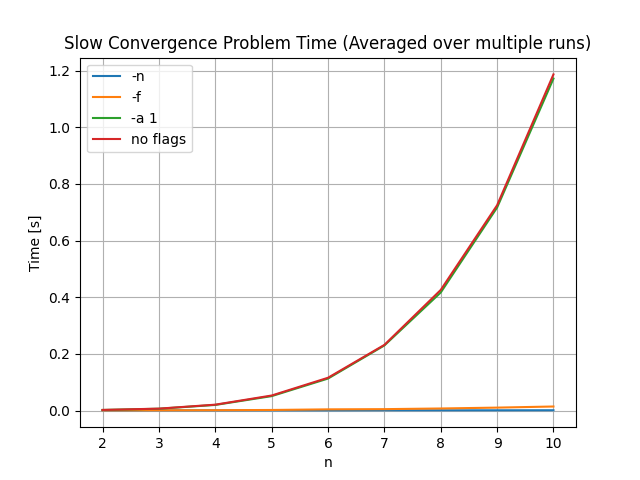
\includegraphics[width=0.8\textwidth]{./Problems/slow_convergence/plots/time_small.png}
	\caption{Slow Convergence Time measurements averaged over multiple runs (at least 10).}
	\label{fig:slow:time-small}
\end{figure}

\begin{figure}[ht]
	\centering
	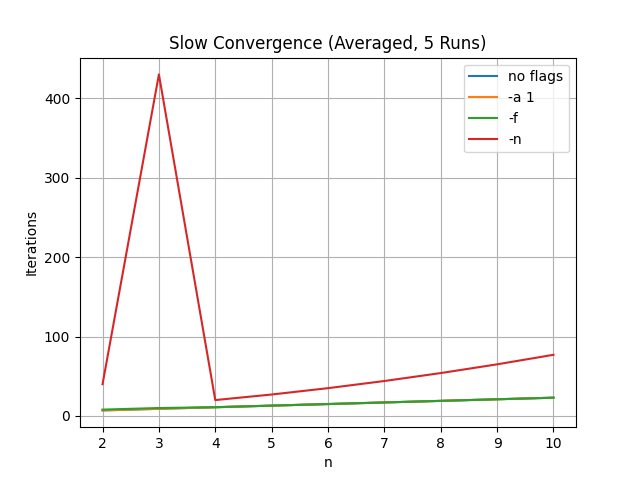
\includegraphics[width=0.8\textwidth]{./Problems/slow_convergence/plots/iterations_small.png}
	\caption{Slow Convergence iteration measurements averaged over 5 runs.}
	\label{fig:slow:iterations-small}
\end{figure}

Next, increasing $n$ for non arc consistency enforcing benchmarks. \cref{fig:slow:sidebyside} shows Time measurements on the left and iteration measurements on the right for $n=10..60$. Note the inverse correlation between Iterations and Time for the two options. Although naive backtracking (\verb|-n|) takes more Iterations, it is still faster than forward checking (\verb|-f|). We can also observe that it looks like forward checking was growing linearly in \cref{fig:slow:time-small}, and \cref{fig:slow:sidebyside} on the left clearly show also exponential growth for forward checking. Further we can again observe that the naive approach seems to be growing linearly, but as we will see, it also grows exponentially.

\begin{figure}[ht]
	\centering
	\begin{minipage}{0.49\textwidth}
		\centering
		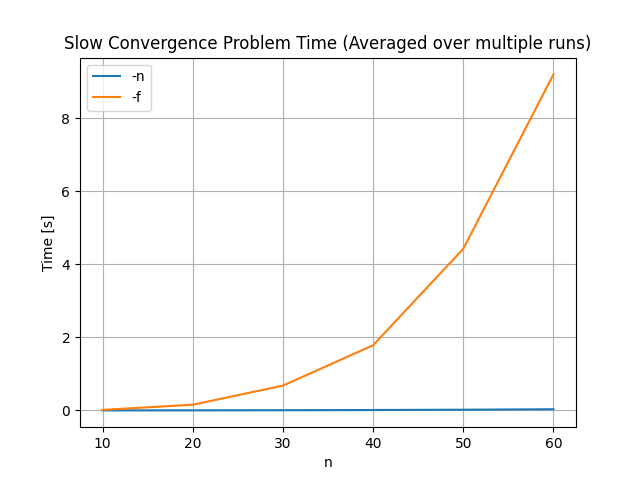
\includegraphics[width=\textwidth]{./Problems/slow_convergence/plots/time.png}
	\end{minipage}
	\hfill
	\begin{minipage}{0.49\textwidth}
		\centering
		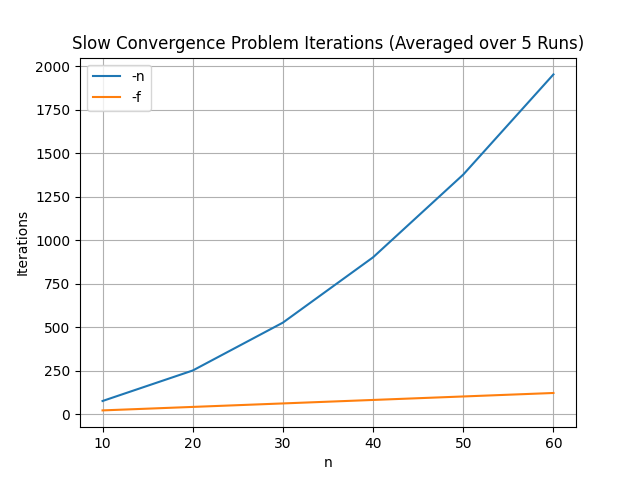
\includegraphics[width=\textwidth]{./Problems/slow_convergence/plots/iterations.png}
	\end{minipage}
	\caption{Comparison for higher $n = 10..60$. Left: Time, right: Iterations.}
	\label{fig:slow:sidebyside}
\end{figure}

\cref{tab:slow:time} and \cref{tab:slow:iterations} contain results for Time and Iterations with standard deviation for the $n = 10..60$ range.

\begin{table}[h!]
	\centering
	\begin{tabular}{c c}
		\begin{minipage}{.5\textwidth}
			\centering
			\begin{tabular}{| c | c | c |}
				\hline
				n  & Naive w/ VO & FC w/ VO        \\ \hline
				10 & 0.00        & 0.01            \\ \hline
				20 & 0.00        & 0.13            \\ \hline
				30 & 0.01        & 0.54 $\pm$ 0.01 \\ \hline
				40 & 0.01        & 1.58 $\pm$ 0.08 \\ \hline
				50 & 0.02        & 5.29 $\pm$ 0.14 \\ \hline
				60 & 0.04        & 21.94 $\pm$ 0.5 \\ \hline
			\end{tabular}
			\caption{Slow Convergence Time in seconds averaged over multiple runs (at least 10), Mean$\pm$SD, w/ VO: with variable ordering.}
			\label{tab:slow:time}
		\end{minipage} &
		\begin{minipage}{.5\textwidth}
			\centering
			\begin{tabular}{| c | c | c |}
				\hline
				n  & Naive w/ VO & FC w/ VO \\ \hline
				10 & 77          & 23       \\ \hline
				20 & 252         & 43       \\ \hline
				30 & 527         & 63       \\ \hline
				40 & 902         & 83       \\ \hline
				50 & 1377        & 103      \\ \hline
				60 & 1952        & 123      \\ \hline
			\end{tabular}
			\caption{Slow Convergence number of Iterations over 5 runs, w/ VO: with variable ordering.}
			\label{tab:slow:iterations}
		\end{minipage}
	\end{tabular}
\end{table}

\section{Gecode}

For comparison \cref{fig:slow:gecode} shows Oxiflex compared to Gecode~\cite{gecode}. Gecode is a CSP solver compatible with MiniZinc with state-of-the art performance. Note the steep increase in $n = 100..600$. And we can again observe that the naive approach grows exponentially.

\begin{figure}[ht]
	\centering
	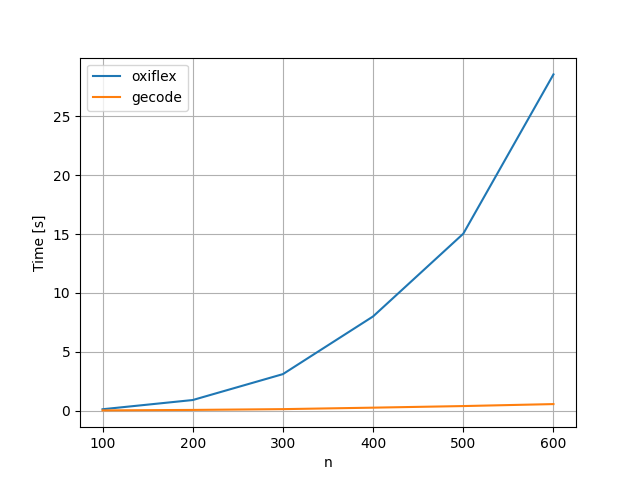
\includegraphics[width=0.8\textwidth]{./Problems/slow_convergence/plots/gecode.png}
	\caption{Slow Convergence Time measurements averaged over multiple runs.}
	\label{fig:slow:gecode}
\end{figure}
